%--------------------
% Packages
% -------------------
\documentclass[11pt,a4paper]{article}
\usepackage[utf8x]{inputenc}
\usepackage[T1]{fontenc}
%\usepackage{gentium}
\usepackage{mathptmx} % Use Times Font


\usepackage{comment}
\usepackage[pdftex]{graphicx} % Required for including pictures
\usepackage[pdftex,linkcolor=black,pdfborder={0 0 0}]{hyperref} % Format links for pdf
\usepackage{calc} % To reset the counter in the document after title page
\usepackage{enumitem} % Includes lists

\frenchspacing % No double spacing between sentences
\linespread{1.2} % Set linespace
\usepackage[a4paper, lmargin=0.1666\paperwidth, rmargin=0.1666\paperwidth, tmargin=0.1111\paperheight, bmargin=0.1111\paperheight]{geometry} %margins
%\usepackage{parskip}

\usepackage[all]{nowidow} % Tries to remove widows
\usepackage[protrusion=true,expansion=true]{microtype} % Improves typography, load after fontpackage is selected

\usepackage{lipsum} % Used for inserting dummy 'Lorem ipsum' text into the template

\usepackage[export]{adjustbox}
\usepackage{plantuml}
\usepackage{float}
\usepackage{indentfirst}
\usepackage{subcaption}

\usepackage{graphicx}

%\usepackage{etoolbox} % Adds '\clearpage' to every '\section command' (newpage).
%\pretocmd{\section}{\clearpage}{}{} 

\newcommand{\inputdiagram}[1]{\input{Diagrams/out/#1}}
\newcommand{\textwidthdiagram}[2][1]{%
  \resizebox{#1\textwidth}{!}{\inputdiagram{#2}}%
}

%-----------------------
% Set pdf information and add title, fill in the fields
%-----------------------
\hypersetup{ 	
pdfsubject = {Program Systems Engineering},
pdftitle = {itssoover},
pdfauthor = {Ignas Časas, Mykolas Marius Budrys, Augustas Kniška}
}

%-----------------------
% Begin document
%-----------------------
\begin{document} %All text i dokumentet hamnar mellan dessa taggar, allt ovanför är formatering av dokumentet

\begin{titlepage}
    \centering
    % Remove page numbering from title
    \thispagestyle{empty}
    
    % University name
    {\Large VILNIAUS UNIVERSITETAS\\
    Matematikos ir informatikos fakultetas}\par
    
    \vspace{3cm} % vertical space
    
    % Title of the work
    {\Large 2\textsuperscript{nd} Laboratory Work}\par
    \vspace{0.5cm}
    {\Large \textbf{itssoover}}\par
    {\Large \textbf{Design and Implementation}}\par
    
    \vspace{3cm}
    
    % Authors
    {\large
    Ignas Časas\\
    Mykolas Marius Budrys\\
    Augustas Kniška
    }\par
    
    \vspace{8cm}
    
    % Bottom of the page
    {\large
    Matematikos ir informatikos fakultetas\\
    Vilniaus universitetas\\
    Lietuva
    }\par
    
    \vfill

    \large 2025
    
\end{titlepage}

\tableofcontents
\newpage

\section{Context}
Our web-based platform offers a number of cognitive games that are designed to test and enhance skills such as memory, attention, reaction time, and problem-solving. Users can access the system directly through a browser without needing to install any software or mobile apps. The platform provides customizable game difficulties and tracks user performance over time. While engaging, the platform prioritizes measurable cognitive improvement over entertainment. 

\subsection{Technology Stack}
\begin{itemize}
    \item \textbf{Frontend:} Built with Blazor for interactive C\#-based UI.
    \item \textbf{Backend:} .NET (C\#) for business logic, user authentication, and statistics tracking.
    \item \textbf{Database:} SQLite for lightweight storage of user data and game progress.
    \item \textbf{Security:} Implements password-protected authentication.
\end{itemize}

\subsection{Content \& Accessibility Boundaries}
\begin{itemize}
    \item Games focus on cognitive improvement, not entertainment or storytelling.
    \item No complex mechanics (e.g., multiplayer or 3D).
    \item Web-based only—no mobile apps, downloads, or third-party integrations.
\end{itemize}

\subsection{Functionality \& Monetization}
\begin{itemize}
    \item Single-player only; no social features.
    \item No in-game purchases or microtransactions.
\end{itemize}



\section{Logical View}


\subsection{Class Diagram}

\begin{figure}[H]
     \centering
     \begin{adjustbox}{width=0.92\paperwidth,center}
+        \inputdiagram{class_diagram.tex}
     \end{adjustbox}
     \caption{Class Diagram}
     \label{fig:class_diagram}
\end{figure}

Figure~\ref{fig:class_diagram} illustrates the structure of the application, dividing it into client-side and server-side components. On the client side, frontend pages inherit from BlazerComponentBase, including AccountPage and StatisticsPage for tracking cognitive progress, SettingsPage for managing privacy settings, and game-specific pages like MathGamePage, SudokuGamePage, PairMatchingGamePage, and AimTrainerPage, all of which utilize TimerService for countdowns. Most .cs files related to these pages are located in the Client/Pages folder, TimerService is located in Client/Services.

On the server side, controllers in the 'Server/Controllers' folder, including AccountScoreController, MathGameController, and others, expose API endpoints. Business logic is handled by services such as MathGameService, SudokuService, AimTrainerService, PairUpService, AccountScoreService, and UserService, all located in the 'Server/Services folder'. Repositories like ScoreRepository and UserRepository in the 'Server/Repositories' folder manage database interactions.

Shared resources include models from the 'Shared/Models' folder and Data Transfer Objects (DTOs) such as UserScoreDto<T> and AverageScoreDto, which facilitate communication between the frontend and backend.

\subsection{Local User States}
\begin{figure}[H]
    \centering
    \begin{minipage}[b]{0.59\textwidth}
        \centering
        \textwidthdiagram{score_fetching_state.tex}
        \caption{Frontend Score Fetching}
        \label{fig:score_fetching_state}
    \end{minipage}
    \hfil
    \begin{minipage}[b]{0.4\textwidth}
        \centering
        \textwidthdiagram{user_authentication_state.tex}
        \caption{User Authentication State}
        \label{fig:user_authentication_state}
    \end{minipage}
\end{figure}

Figure~\ref{fig:score_fetching_state} outlines the asynchronous score
retrieval process happening on the application frontend. This state is kept
when navigating to a game page while authenticated. The state enters in a
"Loading Scores" state where a background call (GetUserHighScoreAsync())
fetches data. Depending on the outcome, the state branches into one
of three paths: it moves to "No Scores Found" if no score is returned,
"Encountered Error" if an error occurs, or "Showing Scores" if the scores
are successfully loaded. The User is shown different UI elements based on
the state. This structure ensures that the application handles different
scenarios gracefully while providing clear feedback to the user.

The User Authentication diagram presented in
Figure~\ref{fig:user_authentication_state} defines the different possible
states of user authentication. The user begins in an "Unauthenticated" state. When a
user attempts to log in, the system remains in the same state if the login
fails, or it transitions to the "Authenticated" state upon a successful
login. A logoff action then reverts the system back to the "Unauthenticated"
state. The defined transitions make asynchronous calls to the Auth API privided
by our back-end solution. This model clearly delineates the transitions
between being logged in and logged out, ensuring that the system maintains
a secure and predictable user session management process.

\subsection{Game States}
\begin{figure}[H]
    \centering
    \begin{minipage}[b]{0.48\textwidth}
        \centering
        \textwidthdiagram{math_state.tex}
        \caption{Math Game State Representation}
        \label{fig:math_state}
    \end{minipage}
    \hfil
    \begin{minipage}[b]{0.48\textwidth}
        \centering
        \textwidthdiagram{aim_trainer_state.tex}
        \caption{Aim Trainer State Representation}
        \label{fig:aim_trainer_state}
    \end{minipage}
\end{figure}

In Figure~\ref{fig:aim_trainer_state} we model our \textit{Aim Training} game. The
game starts by displaying a target, and upon the user's click, it transitions
to a state where the input is processed. If there is remaining time (i.e.,
[time\_left>0]), a new target is generated, looping back to the display state;
otherwise, the game ends. The \textit{ProcessingInput} state handles updating both
the failure count (if the target was missed) and the score.

Figure~\ref{fig:math_state} represents our arithmetic based \textit{Math Game}. It
begins by displaying an equation to the user. When an answer is submitted, the
system transitions to a validation state. The validation state is responsible
for both making an asynchronous call to the back-end for answer validation
and increasing the kept score if the answer was valid. If time remains,
a new question is generated and the process repeats; if not, the game
terminates. Modeling our game in this way highlights the cyclic gameplay
loop that emphasizes both continuous engagement and time-bound gameplay,
ensuring the game session concludes when the allotted time is exhausted.

\begin{figure}[H]
    \centering
    \begin{minipage}[b]{0.48\textwidth}
        \centering
        \textwidthdiagram{sudoku_state.tex}
        \caption{Sudoku State Representation}
        \label{fig:sudoku_state}
    \end{minipage}
    \hfil
    \begin{minipage}[b]{0.48\textwidth}
        \centering
        \textwidthdiagram{pair_up_state.tex}
        \caption{Pair Up State Representation}
        \label{fig:pair_up_state}
    \end{minipage}
\end{figure}

Figure~\ref{fig:sudoku_state} (The \textit{Sudoku} state diagram) captures
the interactive elements of playing our \textit{Sudoku} game. Initially, the board
is idle, waiting for user interaction. When a cell is selected, the state
changes, allowing the user to either deselect the cell, select another
cell, input a value, or submit the board for validation. Upon submission,
the system checks the board (by an asynchronous call to our API): if the
board is invalid, it redraws and returns to the idle state; if the board
is valid, the game ends. These states capture the essential user interactions
and decision points necessary for the logic puzzle.

The \textit{Pair Up} diagram (Figure~\ref{fig:pair_up_state}) details the
states of our memory-based matching game. The game starts with all cards being
shown to the user. The user selects his first card (which the user cannot
unselect), then his second card, prompting the system to evaluate whether the
selected pair matches. If there are still unpaired cards remaining, the game cycles
back to display the cards; if all pairs are successfully matched,
the game ends. This design effectively captures the iterative nature of this
game while clearly defining the conditions for continuation and termination.


\subsection{ER Diagram}

\begin{figure}[H]
    \centering
    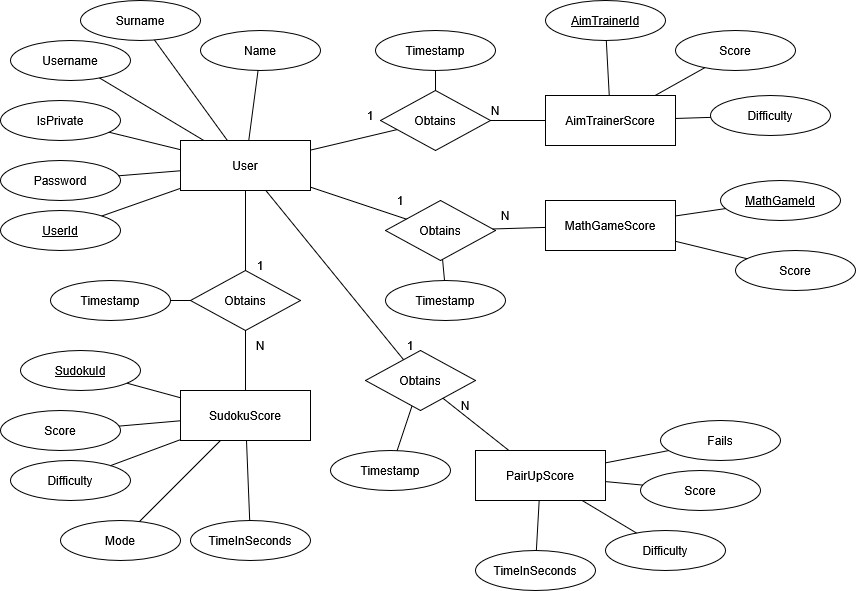
\includegraphics[width=\textwidth]{Diagrams/out/PNG/ER_diagram.png}
    \caption{ER Diagram}
    \label{fig:ER_diagram}
\end{figure}

In Figure~\ref{fig:ER diagram}, the database tables and their relationships are displayed, representing the structure of the system. The diagram models how users interact with different game types and how scores are stored.



\section{Development View}

\subsection{Package Diagram}

\begin{figure}[H]
    \centering
    \textwidthdiagram{Package_Diagram.latex}
    \caption{Package Diagram} 
    \label{fig:united_package}
\end{figure}

Figure~\ref{fig:united_package} provides an overview of the most significant parts of the codebase. This diagram includes some parts of the system that were not mentioned in the class diagram, such as Shared/Enums, Client/Components, and Server/Database. This addition provides a more detailed view of the system.

The diagram is divided into Client, Server, and Shared folders. The Shared package highlights common elements like data models and enumerations that are used across both the frontend and backend, ensuring consistency and reducing redundancy. The arrows indicate dependencies, illustrating how functionality is physically imported from one package to another



\subsection{Component Diagram}

\begin{figure}[H]
    \centering
    \textwidthdiagram{server_component_diagram.latex}
    \caption{Simplified Component Diagram}
    \label{fig:simp_component_diagram}
\end{figure}

Figure~\ref{fig:simp_component_diagram} illustrates the individual component interactions of the app. The Frontend (WebUI and Navigation) interacts with Core Services via APIs for authentication, game data, statistics, and user management. Core Services (Game Controller, Authentication, Statistics, User Management) manage game logic, security, and data, relying on the Persistence layer. The Persistence layer (DAL, Score Repository, User Repository) handles database interactions through a common interface.

\section{Process View}

\begin{figure}[H]
    \centering
     \begin{adjustbox}{width=0.92\paperwidth,center}
+        \inputdiagram{aim_trainer_page_sequence.tex}
     \end{adjustbox}
     \caption{\textit{Aim Trainer} Page Loading Sequence}
    \label{fig:aim_trainer_page_sequence}
\end{figure}
In order to visualize the way in which score fetching works for all of
our games we will do a case analysis on the \textit{Aim Trainer} page.
Figure~\ref{fig:aim_trainer_page_sequence} illustrates the process flow
when a player opens the Aim Trainer page. Initially, the page immediately
requests the username from the authentication provider component. After
this, an initial page is shown to the user with an icon to indicate the fact
that scores are being loaded. Once the username is retrieved and confirmed
not to be null, the page initiates an asynchronous call to the client-side
service to fetch the player's high score. The client service makes an HTTP GET
request to an endpoint provided by the Aim Trainer controller, which, in turn,
invokes the server-side service. The server service interacts with the Score
Repository and User Database Context to locate the corresponding user and
their scores. Depending on whether the user and score exist, the repository
returns either a list of scores or an empty list. The server service then
filters the result to extract the highest score, and this filtered result
is passed back up the chain and sent back as JSON (if a score was found)
and an empty response otherwise. After parsing and unwrapping the data on
the client side, the Aim Trainer page updates its display, showing either the
retrieved high score or a "Not Found" message if no score was found. Finally,
the updated view is presented to the player. This is the way all of our
games implement the score fetching functionality.

TODO: specifying koki objecta grazina?

\begin{figure}[H]
    \centering
     \begin{adjustbox}{width=0.92\paperwidth,center}
+        \inputdiagram{aim_trainer_set_score_sequence.tex}
     \end{adjustbox}
    \caption{Aim Trainer Score Setting Sequence}
    \label{fig:aim_trainer_set_score_sequence}
\end{figure}

This sequence diagram (Figure~\ref{fig:aim_trainer_set_score_sequence}) is an
example of the process initiated by finishing a play session in one our games
\textbf{WHILE AUTHENTICATED} (otherwise no such process occurs on the client
side). Once the game ends, the page calls the client-side service to save the
player's score asynchronously. The client service wraps the score within a
DTO and forwards it via an HTTP POST request to an API endpoint provided by
the Aim Trainer controller. The controller then uses the server-side service
component to process the request. The server-side service unwraps the DTO
and uses an interface provided by the Score Repository, which attempts
to find the corresponding user within the given database context.  If the
user is found, the repository attempts to add the score to the database;
if an exception occurs during this process it is caught by the controller
and the controller decides the appropriate HTTP error code to return (HTTP
500 for DB exceptions, or HTTP 400 when a user is not found, indicating
that a deceptive request might have been sent). If the user is found, and
the insertion process is successful the controller returns a HTTP 200 OK
code. Finally, the result is propagated back through the client service to
the Aim Trainer page, updating the UI accordingly.

\subsection{Activity Diagram}
TODO: Mykolas

\section{Physical View}
\subsection{Deployment}
\begin{figure}[H]
    \centering
    \textwidthdiagram[0.8]{deployment_diagram.tex}
    \caption{Deployment Diagram}
    \label{fig:deployment_diagram}
\end{figure}

TODO: include components

Figure~\ref{fig:deployment_diagram} illustrates the architecture of the web application,
which consists of a client-side Blazor WebAssembly (WASM) front-end and a back-end hosted on an Azure server. The client browser executes the .NET WASM
runtime, running Client.dll as an executable. The backend operates in a Linux
environment within Azure, where the .NET runtime hosts Server.dll. Data is
persisted using an SQLite database. Communication between the client and
server occurs over HTTPS, ensuring secure data transmission. This design
enables a lightweight client while leveraging cloud infrastructure for
back-end processing and storage of user and game data.

\subsection{CI/CD}

\begin{figure}[H]
        \centering
        \textwidthdiagram[0.8]{CI.tex}
        \caption{CI Pipeline}
        \label{fig:CI_pipeline}
\end{figure}
Figure~\ref{fig:CI_pipeline} focuses on our pull request (PR) validation
workflow. Triggered by any pull request targeting the main branch, this
pipeline starts by setting up a linux environment (latest Ubuntu) and
executing a series of steps: checking out the code, setting up the .NET
environment, restoring dependencies, building the solution, and running
tests. The critical decision point here assesses whether all tests pass. If
they do, the PR status is marked as passing, signaling readiness for review
and potential merge. If any tests fail, the pipeline marks the PR as failing
and prevents it from being merged, thus upholding code quality and integrity
before changes are integrated into the main branch.

\begin{figure}[H]
    \centering
    \textwidthdiagram[0.8]{CD.tex}
    \caption{CD Pipeline}
    \label{fig:CD_pipeline}
\end{figure}
Figure~\ref{fig:CD_pipeline} illustrates our CD pipeline using GitHub
Actions. The whole process is excecuted on a linux(latest Ubuntu)
environment. The process begins when a push to the main branch or a manual
trigger starts the pipeline. Within the "Build and Test Job" partition,
the pipeline checks out the repository, sets up the .NET environment,
restores dependencies, and builds the application. After running tests,
the workflow evaluates the outcome: if the tests succeed, it proceeds to
publish the application and upload the resulting artifact; if any test fails,
the deployment is aborted immediately. Following a successful build and test
phase, the "Deploy Job" partition retrieves the artifact from the previous
step and deploys it to Azure, ensuring that only verified code is promoted
to production.

\section{Use Case View}

\begin{figure}[H]
    \centering
    \begin{minipage}[b]{0.48\textwidth}
        \centering
        \textwidthdiagram{use_case_account.tex}
        \caption{Account Use Case}
        \label{fig:use_case_account}
    \end{minipage}
    \hfil
    \begin{minipage}[b]{0.48\textwidth}
        \centering
        \textwidthdiagram{use_case_game_page.tex}
        \caption{Game Page}
        \label{fig:use_case_game_page}
    \end{minipage}
\end{figure}

Figure~\ref{fig:use_case_account} shows how players interact with the Account module.
Unauthenticated players can log in or sign up, while authenticated players can log out.

Figure~\ref{fig:use_case_game_page} outlines two key actions: starting a game and
changing the difficulty level. This design ensures that players have direct
control over initiating gameplay and tailoring the challenge to their
preferences.

\begin{figure}[H]
    \centering
    \begin{minipage}[b]{0.48\textwidth}
        \textwidthdiagram{use_case_high_score.tex}
        \caption{High Score Module}
        \label{fig:use_case_high_score}
    \end{minipage}
    \hfil
    \begin{minipage}[b]{0.48\textwidth}
        \centering
        \textwidthdiagram{use_case_navigation.tex}
        \caption{Page Navigation}
        \label{fig:use_case_navigation}
    \end{minipage}
\end{figure}

Figure~\ref{fig:use_case_high_score} details various ways for authenticated players to review game performance. Users
can view short game statistics, detailed graphs, timelines of past games, and
statistics filtered by difficulty. The module provides multiple perspectives to
help players track and analyze their performance.

Figure~\ref{fig:use_case_navigation} maps out the main paths for navigating through the website.
Players can easily switch between the home page (which doubles as the game
selection page), the account page, and the statistics page, ensuring a
user-friendly and integrated browsing experience.

\begin{figure}[H]
    \begin{minipage}[b]{0.48\textwidth}
        \centering
        \textwidthdiagram{use_case_game_selection.tex}
        \caption{Game selection}
        \label{fig:use_case_game_selection}
    \end{minipage}
    \hfil
    \begin{minipage}[b]{0.48\textwidth}
        \centering
        \textwidthdiagram{use_case_settings.tex}
        \caption{Account Settings}
        \label{fig:use_case_settings}
    \end{minipage}
\end{figure}
Figure~\ref{fig:use_case_game_selection} illustrates the available games that
players can choose from. Players can select one of four games: Aim Trainer,
Math Game, Pair Up, or Sudoku. This selection allows users to navigate to
a game page based on their preferences.

Figure~\ref{fig:use_case_settings} shows the settings available to
authenticated players. Users can choose to make their high scores public
or keep them private. This feature provides control over personal game
performance visibility, enhancing user privacy options.


\section{Traceability}
\begin{table}[H]
\begin{tabular}{|l|l|}
\hline
\multicolumn{1}{|c|}{\textbf{User Needs}}    & \multicolumn{1}{|c|}{\textbf{Requirements}}                   \\ \hline
\multicolumn{2}{|c|}{\textbf{Players (Primary stakeholder)}}                                           \\ \hline
Ease of Access (1.a)                         & F 1.a (Web-based application)                \\
Variety of Games (1.b)                       & F 2.b (Display a variety of cognitive games), F 3 (Games) \\
User Account (1.c)                           & F 2.a (Allow users to log in or sign up)     \\
Progress Tracking (1.d)                      & F 4.e (Scoreboard for tracking progress)     \\
Ranking System (1.e)                         & F 4.g (Update leaderboards after game)       \\
Personalization (1.f)                        & F 4.b (Difficulty settings for games)        \\
User-Friendly Interface (1.g)                & F 2 (Main Menu Page), NF 4 (Compatibility)   \\
Game Description (1.h)                       & F 4.a (Each game must have a description)    \\
\hline
\multicolumn{2}{|c|}{\textbf{Developers (Primary Stakeholders)}}                                       \\
\hline
\colorbox{yellow}{Clear Requirements \& Design (2.a)}           & \colorbox{yellow}{F 5.a (Functional \& technical specifications)} \\
\colorbox{yellow}{Documentation (2.b)   }                       & \colorbox{yellow}{F 5.b (Code docs \& technical docs)  }        \\
Testing Environment (2.c)                   & 
F 5.c (Testing setup with CI integration)    \\
\hline
\multicolumn{2}{|c|}{\textbf{Administrators (Primary Stakeholders)}}                                   \\
\hline
User Management (3.a)                 &  F 2.c (Privacy settings for leaderboard)    \\
\colorbox{yellow}{Game and Content Management (3.b)}            & \colorbox{yellow}{F 4 (User Experience Enhancements)  }         \\
\colorbox{yellow}{System Monitoring (3.c)}   & \colorbox{yellow}{NF 2.b (Logging \& real-time monitoring), NF 3.a (Security)} \\
\hline
\multicolumn{2}{|c|}{\textbf{Shareholders / Investors (Primary Stakeholders)}}                         \\
\hline
\colorbox{yellow}{Profitability \& Growth (4.a) }               & \colorbox{yellow}{NF 1 (Performance requirements)  }            \\
\colorbox{yellow}{Project Stability (4.b) }                     & \colorbox{yellow}{NF 2.a (90\% system uptime)}                  \\
Reports and Statistics (4.c)                 & F 4.e (User performance tracking)            \\
\hline
\multicolumn{2}{|c|}{\textbf{Partners - Educational Institutions (Secondary Stakeholders)}}            \\
\hline
Accessibility \& Reliability (5.a)           & NF 4 (Compatibility), NF 1 (Performance)     \\
Data Analysis (5.b)                          & F 4.e (Tracking progress \& game statistics) \\
Integration into Learning Process (5.c)      & F 4.a (Descriptions of game's benefits)      \\
\hline
\multicolumn{2}{|c|}{\textbf{National Institute of Standards and Technology (Secondary Stakeholders)}} \\
\hline
\colorbox{yellow}{Password Security \& Encryption (6.a)}        & \colorbox{yellow}{NF 3 (Security)  }                            \\
\hline
\multicolumn{2}{|c|}{\textbf{Compliance with local laws - GDPR (Secondary Stakeholders)}}              \\
\hline
\colorbox{yellow}{Data Protection Principles (7.a) }             &\colorbox{yellow}{ NF 5.d (Data Protection Principles) }         \\
\colorbox{yellow}{Consent Management (7.b)   }                  & \colorbox{yellow}{NF 5.e (Consent Management)  }                \\
\colorbox{yellow}{Data Subject Rights (7.c)  }                  & \colorbox{yellow}{NF 5.f (Data Subject Rights) }                \\
\hline
\end{tabular}

\vspace{8pt} % value to increase the gap

\textbf{F (Functional Requirements), NF (Non-Functional Requirements)}

\vspace{8pt} % value to increase the gap

\textbf{Note:} The current system architecture does not follow or implement user needs and requirements highlighted in yellow. All other unmarked requirements and user needs are either mentioned in the system or have some form of implementation that can be checked. Unmarked columns are mentioned in the system architecture diagrams.
\end{table}


%\lipsum[1-3]



\end{document}
